% Set options for wide aspect ratio and beamer document class
\documentclass[aspectratio=169]{beamer}

% Package imports
\usepackage{fontspec}
\usepackage{epigraph}
\usepackage{xcolor}
\usepackage[percent]{overpic}
\usepackage{pgfpages}

% custom options to make epigraph look good on a beamer slide
\renewcommand{\epigraphrule}{0pt}
\setlength{\epigraphwidth}{.9\textwidth}
\renewcommand{\textflush}{flushepinormal}

\newcommand\blfootnote[1]{%
  \begingroup
  \renewcommand\thefootnote{}\footnote{#1}%
  \addtocounter{footnote}{-1}%
  \endgroup
}

% default document font specifications
\setmainfont{FiraSans-Book}
\setsansfont{FiraSans-Book}
\definecolor{textcolour}{rgb}{255,255,255}

% Definign the Mozilla colour palette for presentations 
\definecolor{moz_dark_green}{RGB}{77,78,83}
\definecolor{moz_light_green}{RGB}{208,211,212}
\definecolor{moz_light_blue}{RGB}{0,150,221}
\definecolor{moz_dark_blue}{RGB}{0,33,71}
\definecolor{moz_accent_green}{RGB}{111,190,74}
\definecolor{moz_accent_yellow}{RGB}{255,203,0}
\definecolor{moz_accent_orange}{RGB}{255,149,0}
\definecolor{moz_accent_orange2}{RGB}{230,96,0}
\definecolor{moz_accent_red}{RGB}{193,56,50}

% new counter for column enumerates
\newcounter{savedenum}
\newcommand*{\saveenum}{\setcounter{savedenum}{\theenumi}}
\newcommand*{\resume}{\setcounter{enumi}{\thesavedenum}}

% Background for all slides set here
\setbeamertemplate{background canvas}{
\includegraphics [width=\paperwidth]{bg_black.png}}

\setbeamercolor{structure}{fg=textcolour}

\setbeamerfont{title}{size = \Huge}
\setbeamercolor{normal text}{fg=textcolour}

%define specific fint size interpretations for the beamer presentation mode.
\renewcommand{\tiny}{\fontsize{7pt}{8pt}\selectfont}
\renewcommand{\scriptsize}{\fontsize{9pt}{12pt}\selectfont}
\renewcommand{\footnotesize}{\fontsize{10pt}{12pt}\selectfont}
\renewcommand{\small}{\fontsize{12pt}{18pt}\selectfont}
\renewcommand{\normalsize}{\fontsize{14pt}{18pt}\selectfont}
\renewcommand{\large}{\fontsize{16pt}{24pt}\selectfont}
\renewcommand{\Large}{\fontsize{24pt}{37pt}\selectfont}
\renewcommand{\LARGE}{\fontsize{31pt}{42pt}\selectfont}
\renewcommand{\huge}{\fontsize{48pt}{54pt}\selectfont}
\renewcommand{\Huge}{\fontsize{80pt}{96pt}\selectfont}

% remove navigation symbols
\setbeamertemplate{navigation symbols}{}
 
% After building the PDF you may ensure that local system fonts are embedded in the final PDF using:
% gs -dNOPAUSE -dBATCH -sDEVICE=pdfwrite -dPDFSETTINGS=/prepress -dEmbedAllFonts=true -sOutputFile=DN2018-lopatka-portable.pdf -f DN2018-Lopatka.pdf
% This will also compress the final output size 

%\setbeameroption{show notes}
%\setbeameroption{show notes on second screen}

\begin{document}

%% slide 1
\begin{frame}
\begin{overpic}[width=0.7\textwidth]{taar2_compressed.png}
\end{overpic}
%% Speaker notes:
\note{
	\begin{itemize} 
		\item{Personalised web browsing experience is hard}
		\item{Especially with a rigorous and respectful privacy policy}
		\item{Ultimately, many of the approaches in UMAP strive to find innovative ways to extract a meaningful signal from very noisy data.}
	\end{itemize}
}
%%
\end{frame}

%% slide 2
{
\usebackgroundtemplate{\includegraphics[width=\paperwidth]{bg_alt_small-rlogo.png}}
\begin{frame}
\begin{overpic}[width=0.7\textwidth]{taar1_compressed.png}
\put(85, 7){\large{Martin Lopatka}}
\put(78, 1){\small{mlopatka@mozilla.com}}
\put(57.25, -5){\small{Data Scientist/Applied Statistician}}
\end{overpic}
%% Speaker notes:
\note{
    \begin{itemize}
        \item{Martin Lopatka}
        \item{Time we have through... Mozilla's approach to recommending browser extensions}
        \item{T.A.A.R.}
        \item{Curiosity vs. builders }
        \item{given the time, focus on a very brief overview, and two specific design choices}
        \item{Privacy by design and CLLR}
\end{itemize}
}
%
\end{frame}
}

{
\usebackgroundtemplate{\includegraphics[width=\paperwidth]{bg_alt_small-rlogo.png}}
\begin{frame}
\frametitle{Telemetry}
\begin{center}\large{Firefox Telemetry (optionally) measures and collects non-personal, performance and usage information.}\footnote{https://wiki.mozilla.org/Telemetry}\end{center}
%% Speaker notes:
    \note{
        \begin{itemize}
\item{application localization identifier: (ch-de, br-pt)}
\item{operating system}
\item{subsession length}
\item{bookmark count}
\item{open tab count}
\item{unique TLDs}
\item{add-ons installed}
        \end{itemize}
    }
%
\end{frame}
}

{
\usebackgroundtemplate{\includegraphics[width=\paperwidth]{bg_alt_small-rlogo.png}}
\begin{frame}
\frametitle{Telemetry-Aware Add-on Recommender}
\begin{center}\includegraphics[width=0.8\textwidth]{taar-flow.png}\end{center}
%% Speaker notes:
    \note{
        \begin{itemize}
        \item{Full system Spec} 
        \item{Three modules each leveraging different subsets of client information based on availability.} 
        \item{Individual recommendations combined via linear stacked ensemble}
        \item{These are domain specific and specific to our telemetry infra, so lets treat them like black boxes}
        \item{more interesting is the comparison of functions for determining individual weighting of the recommendations.}     
        \end{itemize}
    }
%
\end{frame}
}

{
\usebackgroundtemplate{
\includegraphics[width=\paperwidth]{LR-bg.jpg}}
\begin{frame}
\frametitle{Differential Privacy}
\begin{itemize}
\item{Differentially private release mechanism for frequencies reports an approximate answer to an \textbf{\textit{item:count}} distribution.}
\item{Noise must be chosen to preserve the usefulness of the provided answer while protecting the privacy of the more rare counts}
\end{itemize}
\vspace{0.5cm}
\tiny{Introduction to DP: https://robertovitillo.com/2016/07/29/differential-privacy-for-dummies/}
%% Speaker notes:
    \note{
        \begin{itemize}
        \item{Formalizes the idea that released data set can not be used to infer whether any one person is present}
        \item{Typically generated on the basis of a known distribution and some known noise distribution.} 
        \item{We adapt this technique to generate add-on installation frequency tables for each locale according to the following procedure}
        \item{Guards against Overfitting}        
        \end{itemize}
    }
%
\end{frame}
}

{
\usebackgroundtemplate{
\includegraphics[width=\paperwidth]{LR-bg.jpg}}
\begin{frame}
\frametitle{Log Likelihood Ratio Cost (cLLR)}
\footnotesize{\texttt{\noindent'zh-CN': [('guid\_01', 0.75),...,('guid\_02', 0.05)],\\
\noindent'fr-FR': [('guid\_03', 0.24),...,('guid\_04', 0.01)],\\
\noindent...,\\
\noindent'en-US': [('guid\_04', 0.18),...,(guid\_05', 0.02)]
}}
\begin{center}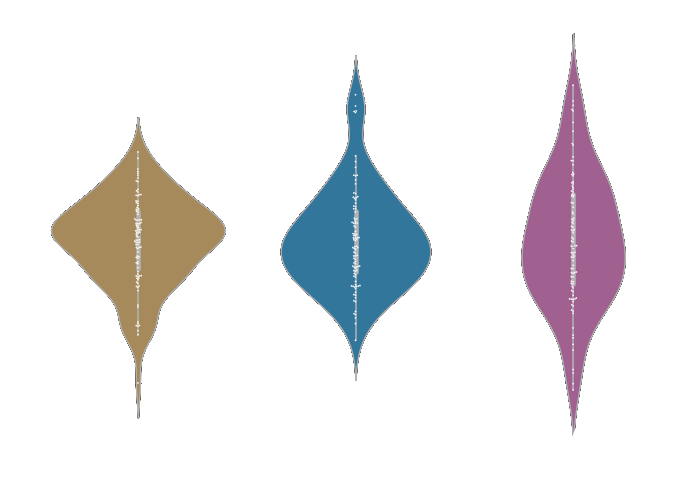
\includegraphics[width=0.6\textwidth]{vio-plots-optimize.png}\end{center}

%% Speaker notes:
\note{
        \begin{itemize}
        \item{better usage of full signal if component modules a probabilistic (flavoured) ignores rank!}
        \item{reference keynote, choosing the *correct* metric}
        \item{Symmetry accounts for incorrect recommendations (instead of just relative rank fo correct recommendations and the relevance score)}        
        \item{Versus Discounted Cumulative Gain (DCG), and versus Mean Average Precision (MAP) for including in the recommendation list at all}
        \end{itemize}
    }
%
\end{frame}
}

{
\usebackgroundtemplate{
\includegraphics[width=\paperwidth]{LR-bg.jpg}}
\begin{frame}
\frametitle{Experimental design}
Experiment ran: 27-Aug-2018 to 29-Oct-2018\\
Served recommendations to 348 900 unique clients\\

\begin{itemize}
\item{\textbf{control} — Manually curated list of add-ons based on a user’s locale}
\item{\textbf{ensemble} — Weighted combination of all eligible models from the TAAR service}
\item{\textbf{hybrid} — Identical to the ensemble with some curated add-ons interleaved}
\end{itemize}
%% Speaker notes:
\note{
        \begin{itemize}
        \item{better usage of full signal if component modules a probabilistic (flavoured)}
        \item{Symmetry also accounts for incorrect recommendations (instead of just relative rank fo correct recommendations and the relevance score)}        
        \item{Versus Discounted Cumulative Gain (DCG), and versus Mean Average Precision (MAP) for including in the recommendation list at all}
        \end{itemize}
    }
%
\end{frame}
}

{
\usebackgroundtemplate{\includegraphics[width=\paperwidth]{bg_alt_small-rlogo.png}}
\begin{frame}
\frametitle{Performance}
\vspace{-1.5cm}
\begin{center}\includegraphics[width=1.05\textwidth]{taar-all-performance.png}\end{center}
%% Speaker notes:
    \note{
        \begin{itemize}
        \item{variable availability of our data, not only in terms of quantity but in terms of fields}
        \item{handles peculiar data sparsity problems well}
        \item{Performs well and scales with data availability}
        \item{And 100\% open source} 
        \item{TAAR Serves about 240K recommendations per day in under 100ms}
        \end{itemize}
    }
%
\end{frame}
}

{
\usebackgroundtemplate{\includegraphics[width=\paperwidth]{bg_alt_small-rlogo.png}}
\begin{frame}
\frametitle{Acknowledgements}
   \begin{columns}
     \begin{column}{.33\linewidth}
Victor Ng\\
Ben Miroglio\\
David Zeber\\
Alessio Placitelli\\
Laura Thomson
     \end{column}
     \begin{column}{.33\linewidth}
Fredrik Wollsén\\
Jason Thomas\\
Stuart Colville\\
Shell Escalante\\
Scott DeVaney\\
Kev Needham
     \end{column}
     \begin{column}{.33\linewidth}
AMO team\\
Localisation team\\
InfoSec\\
QA team\\
Florian Hartmann\\
Roberto Vitillo
     \end{column}
     
   \end{columns}

%% Speaker notes:
    \note{
        \begin{itemize}
        \item{Thank you all for choosing to come engage with me here}
        \item{I'll be happy... questions}        
        \item{but first... acknowledgements}        
        \end{itemize}
    }
%
\end{frame}
}
%% end of presentation
\end{document}